%\subsection{Karush Kuhn-Tucker Conditions}
\begin{problem}
\label{ch1_lp1}
	Graphically obtain a solution to the following 
	\begin{align}
\max_{\mbf{x}}	6x_1 + 5x_2
	\end{align}
	with constraints
	\begin{align}
	x_1 + x_2 &\leq 5\\
	3x_1 + 2x_2 &\leq 12\\
	\text{ where } x_1,x_2 &\geq 0
	\end{align}
\end{problem}
%
\solution
The following program plots the solution in Fig. \ref{fig.4.1}
%	
\lstinputlisting{./chapter4/codes/4.1.py}
%
\begin{figure}[h]
\centering
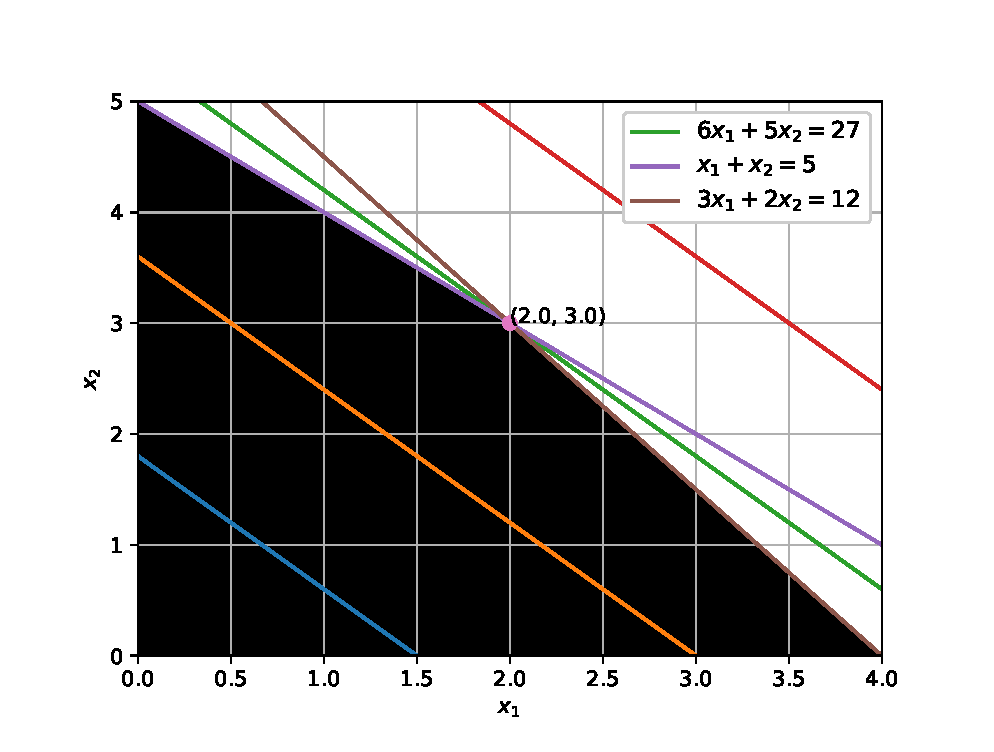
\includegraphics[width=\columnwidth]{./chapter4/figs/4.1.eps}
\caption{ The cost function intersects with the two constraints at $\mbf{x} = \brak{2,3}$. }
\label{fig.4.1}	
\end{figure}
%
\begin{problem}
	Now use {\em cvxopt} to obtain a solution to problem \ref{ch1_lp1}.
\end{problem}
\solution
The given problem is expressed as follows
%
\begin{align}
\min_{\mbf{x}}	\mbf{c}^{T}\mbf{x}\quad s.t.
\\
\mbf{A}\mbf{x} \preceq \mbf{b}
\end{align}
%
where
%
\begin{equation}
\mbf{c}
=
\begin{pmatrix}
-6
\\
-5
\end{pmatrix},
\mbf{A} = 
\begin{pmatrix}
1 & 1
\\
3 & 2
\\
-1 & 0
\\
0 & -1
\end{pmatrix},
\mbf{b}
= 
\begin{pmatrix}
5
\\
12
\\
0
\\
0 
\end{pmatrix}
\end{equation}
%	
The desired solution is then obtained using the following program.
\lstinputlisting{./chapter4/codes/4.2.py}
%
\begin{problem}
	Verify your solution to the above problem using the method of Lagrange multipliers.
\end{problem}
%
\begin{problem}
	 Maximise $5x_1 + 3x_2$ w.r.t the constraints
	 \begin{align}
	 x_1 + x_2 &\leq 2 \nonumber\\
	 5x_1 + 2x_2 &\leq 10 \nonumber\\
	 3x_1 + 8x_2 &\leq 12 \nonumber\\
	 \text{ where } x_1,x_2 &\geq 0 \nonumber
	 \end{align}	
\end{problem}


